\documentclass[1p]{elsarticle_modified}
%\bibliographystyle{elsarticle-num}

%\usepackage[colorlinks]{hyperref}
%\usepackage{abbrmath_seonhwa} %\Abb, \Ascr, \Acal ,\Abf, \Afrak
\usepackage{amsfonts}
\usepackage{amssymb}
\usepackage{amsmath}
\usepackage{amsthm}
\usepackage{scalefnt}
\usepackage{amsbsy}
\usepackage{kotex}
\usepackage{caption}
\usepackage{subfig}
\usepackage{color}
\usepackage{graphicx}
\usepackage{xcolor} %% white, black, red, green, blue, cyan, magenta, yellow
\usepackage{float}
\usepackage{setspace}
\usepackage{hyperref}

\usepackage{tikz}
\usetikzlibrary{arrows}

\usepackage{multirow}
\usepackage{array} % fixed length table
\usepackage{hhline}

%%%%%%%%%%%%%%%%%%%%%
\makeatletter
\renewcommand*\env@matrix[1][\arraystretch]{%
	\edef\arraystretch{#1}%
	\hskip -\arraycolsep
	\let\@ifnextchar\new@ifnextchar
	\array{*\c@MaxMatrixCols c}}
\makeatother %https://tex.stackexchange.com/questions/14071/how-can-i-increase-the-line-spacing-in-a-matrix
%%%%%%%%%%%%%%%

\usepackage[normalem]{ulem}

\newcommand{\msout}[1]{\ifmmode\text{\sout{\ensuremath{#1}}}\else\sout{#1}\fi}
%SOURCE: \msout is \stkout macro in https://tex.stackexchange.com/questions/20609/strikeout-in-math-mode

\newcommand{\cancel}[1]{
	\ifmmode
	{\color{red}\msout{#1}}
	\else
	{\color{red}\sout{#1}}
	\fi
}

\newcommand{\add}[1]{
	{\color{blue}\uwave{#1}}
}

\newcommand{\replace}[2]{
	\ifmmode
	{\color{red}\msout{#1}}{\color{blue}\uwave{#2}}
	\else
	{\color{red}\sout{#1}}{\color{blue}\uwave{#2}}
	\fi
}

\newcommand{\Sol}{\mathcal{S}} %segment
\newcommand{\D}{D} %diagram
\newcommand{\A}{\mathcal{A}} %arc


%%%%%%%%%%%%%%%%%%%%%%%%%%%%%5 test

\def\sl{\operatorname{\textup{SL}}(2,\Cbb)}
\def\psl{\operatorname{\textup{PSL}}(2,\Cbb)}
\def\quan{\mkern 1mu \triangleright \mkern 1mu}

\theoremstyle{definition}
\newtheorem{thm}{Theorem}[section]
\newtheorem{prop}[thm]{Proposition}
\newtheorem{lem}[thm]{Lemma}
\newtheorem{ques}[thm]{Question}
\newtheorem{cor}[thm]{Corollary}
\newtheorem{defn}[thm]{Definition}
\newtheorem{exam}[thm]{Example}
\newtheorem{rmk}[thm]{Remark}
\newtheorem{alg}[thm]{Algorithm}

\newcommand{\I}{\sqrt{-1}}
\begin{document}

%\begin{frontmatter}
%
%\title{Boundary parabolic representations of knots up to 8 crossings}
%
%%% Group authors per affiliation:
%\author{Yunhi Cho} 
%\address{Department of Mathematics, University of Seoul, Seoul, Korea}
%\ead{yhcho@uos.ac.kr}
%
%
%\author{Seonhwa Kim} %\fnref{s_kim}}
%\address{Center for Geometry and Physics, Institute for Basic Science, Pohang, 37673, Korea}
%\ead{ryeona17@ibs.re.kr}
%
%\author{Hyuk Kim}
%\address{Department of Mathematical Sciences, Seoul National University, Seoul 08826, Korea}
%\ead{hyukkim@snu.ac.kr}
%
%\author{Seokbeom Yoon}
%\address{Department of Mathematical Sciences, Seoul National University, Seoul, 08826,  Korea}
%\ead{sbyoon15@snu.ac.kr}
%
%\begin{abstract}
%We find all boundary parabolic representation of knots up to 8 crossings.
%
%\end{abstract}
%\begin{keyword}
%    \MSC[2010] 57M25 
%\end{keyword}
%
%\end{frontmatter}

%\linenumbers
%\tableofcontents
%
\newcommand\colored[1]{\textcolor{white}{\rule[-0.35ex]{0.8em}{1.4ex}}\kern-0.8em\color{red} #1}%
%\newcommand\colored[1]{\textcolor{white}{ #1}\kern-2.17ex	\textcolor{white}{ #1}\kern-1.81ex	\textcolor{white}{ #1}\kern-2.15ex\color{red}#1	}

{\Large $\underline{12a_{1154}~(K12a_{1154})}$}

\setlength{\tabcolsep}{10pt}
\renewcommand{\arraystretch}{1.6}
\vspace{1cm}\begin{tabular}{m{100pt}>{\centering\arraybackslash}m{274pt}}
\multirow{5}{120pt}{
	\centering
	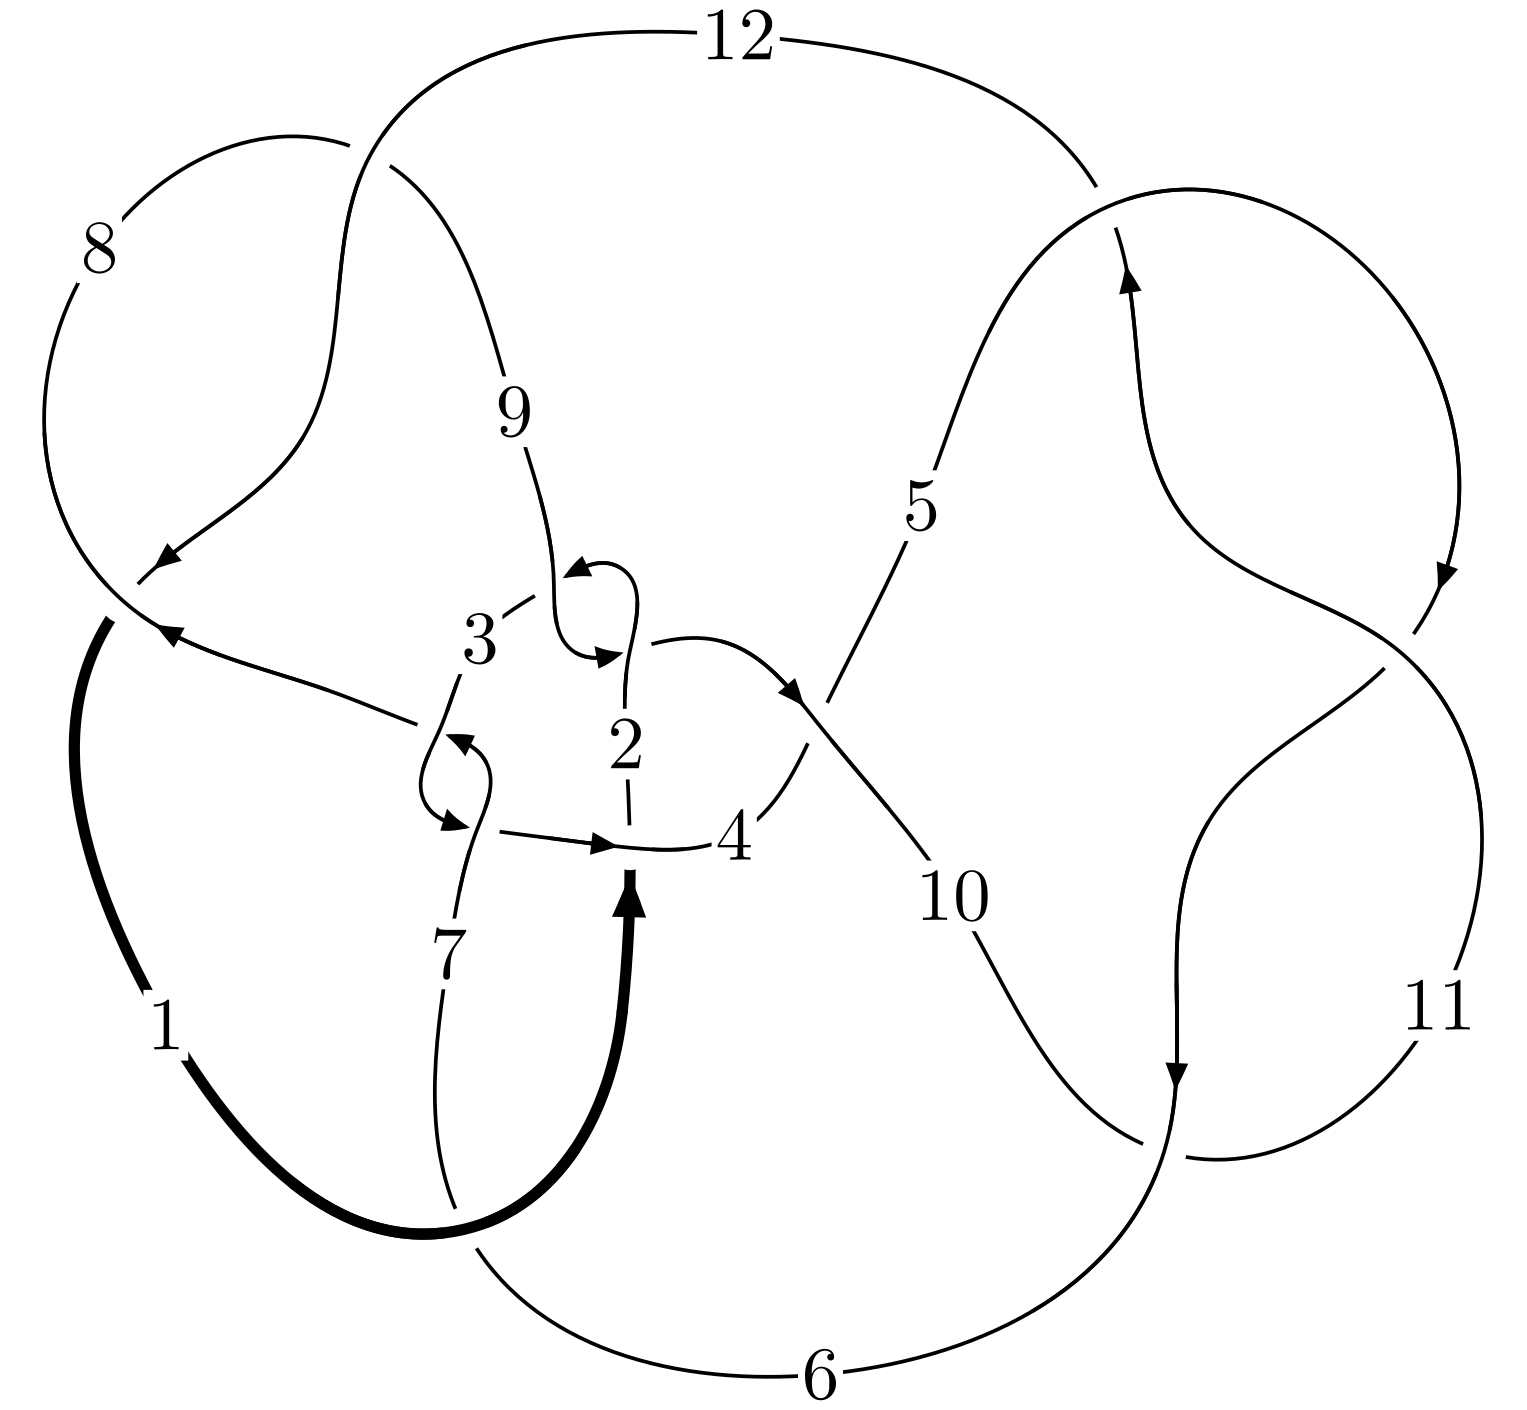
\includegraphics[width=112pt]{../../../GIT/diagram.site/Diagrams/png/1955_12a_1154.png}\\
\ \ \ A knot diagram\footnotemark}&
\allowdisplaybreaks
\textbf{Linearized knot diagam} \\
\cline{2-2}
 &
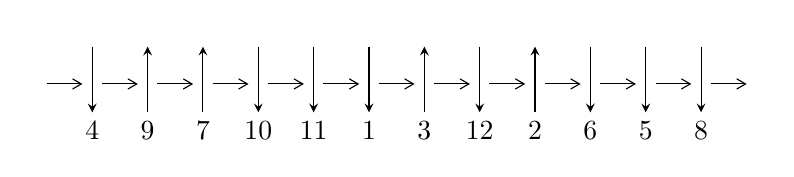
\begin{tikzpicture}[x=20pt, y=17pt]
	% nodes
	\node (C0) at (0, 0) {};
	\node (C1) at (1, 0) {};
	\node (C1U) at (1, +1) {};
	\node (C1D) at (1, -1) {4};

	\node (C2) at (2, 0) {};
	\node (C2U) at (2, +1) {};
	\node (C2D) at (2, -1) {9};

	\node (C3) at (3, 0) {};
	\node (C3U) at (3, +1) {};
	\node (C3D) at (3, -1) {7};

	\node (C4) at (4, 0) {};
	\node (C4U) at (4, +1) {};
	\node (C4D) at (4, -1) {10};

	\node (C5) at (5, 0) {};
	\node (C5U) at (5, +1) {};
	\node (C5D) at (5, -1) {11};

	\node (C6) at (6, 0) {};
	\node (C6U) at (6, +1) {};
	\node (C6D) at (6, -1) {1};

	\node (C7) at (7, 0) {};
	\node (C7U) at (7, +1) {};
	\node (C7D) at (7, -1) {3};

	\node (C8) at (8, 0) {};
	\node (C8U) at (8, +1) {};
	\node (C8D) at (8, -1) {12};

	\node (C9) at (9, 0) {};
	\node (C9U) at (9, +1) {};
	\node (C9D) at (9, -1) {2};

	\node (C10) at (10, 0) {};
	\node (C10U) at (10, +1) {};
	\node (C10D) at (10, -1) {6};

	\node (C11) at (11, 0) {};
	\node (C11U) at (11, +1) {};
	\node (C11D) at (11, -1) {5};

	\node (C12) at (12, 0) {};
	\node (C12U) at (12, +1) {};
	\node (C12D) at (12, -1) {8};
	\node (C13) at (13, 0) {};

	% arrows
	\draw[->,>={angle 60}]
	(C0) edge (C1) (C1) edge (C2) (C2) edge (C3) (C3) edge (C4) (C4) edge (C5) (C5) edge (C6) (C6) edge (C7) (C7) edge (C8) (C8) edge (C9) (C9) edge (C10) (C10) edge (C11) (C11) edge (C12) (C12) edge (C13) ;	\draw[->,>=stealth]
	(C1U) edge (C1D) (C2D) edge (C2U) (C3D) edge (C3U) (C4U) edge (C4D) (C5U) edge (C5D) (C6U) edge (C6D) (C7D) edge (C7U) (C8U) edge (C8D) (C9D) edge (C9U) (C10U) edge (C10D) (C11U) edge (C11D) (C12U) edge (C12D) ;
	\end{tikzpicture} \\
\hhline{~~} \\& 
\textbf{Solving Sequence} \\ \cline{2-2} 
 &
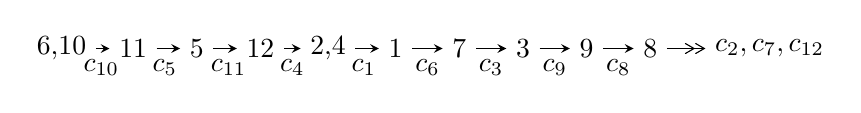
\begin{tikzpicture}[x=23pt, y=7pt]
	% node
	\node (A0) at (-1/8, 0) {6,10};
	\node (A1) at (1, 0) {11};
	\node (A2) at (2, 0) {5};
	\node (A3) at (3, 0) {12};
	\node (A4) at (65/16, 0) {2,4};
	\node (A5) at (41/8, 0) {1};
	\node (A6) at (49/8, 0) {7};
	\node (A7) at (57/8, 0) {3};
	\node (A8) at (65/8, 0) {9};
	\node (A9) at (73/8, 0) {8};
	\node (C1) at (1/2, -1) {$c_{10}$};
	\node (C2) at (3/2, -1) {$c_{5}$};
	\node (C3) at (5/2, -1) {$c_{11}$};
	\node (C4) at (7/2, -1) {$c_{4}$};
	\node (C5) at (37/8, -1) {$c_{1}$};
	\node (C6) at (45/8, -1) {$c_{6}$};
	\node (C7) at (53/8, -1) {$c_{3}$};
	\node (C8) at (61/8, -1) {$c_{9}$};
	\node (C9) at (69/8, -1) {$c_{8}$};
	\node (A10) at (11, 0) {$c_{2},c_{7},c_{12}$};

	% edge
	\draw[->,>=stealth]	
	(A0) edge (A1) (A1) edge (A2) (A2) edge (A3) (A3) edge (A4) (A4) edge (A5) (A5) edge (A6) (A6) edge (A7) (A7) edge (A8) (A8) edge (A9) ;
	\draw[->>,>={angle 60}]	
	(A9) edge (A10);
\end{tikzpicture} \\ 

\end{tabular} \\

\footnotetext{
The image of knot diagram is generated by the software ``\textbf{Draw programme}" developed by Andrew Bartholomew(\url{http://www.layer8.co.uk/maths/draw/index.htm\#Running-draw}), where we modified some parts for our purpose(\url{https://github.com/CATsTAILs/LinksPainter}).
}\phantom \\ \newline 
\centering \textbf{Ideals for irreducible components\footnotemark of $X_{\text{par}}$} 
 
\begin{align*}
I^u_{1}&=\langle 
1.09583\times10^{187} u^{124}+1.47205\times10^{187} u^{123}+\cdots+1.32214\times10^{187} b-3.17493\times10^{187},\\
\phantom{I^u_{1}}&\phantom{= \langle  }2.48538\times10^{188} u^{124}+1.28444\times10^{188} u^{123}+\cdots+3.04093\times10^{188} a+2.28676\times10^{189},\\
\phantom{I^u_{1}}&\phantom{= \langle  }u^{125}+u^{124}+\cdots+19 u-23\rangle \\
I^u_{2}&=\langle 
2 u^{26}+27 u^{24}+\cdots+b+2,\;- u^{26}-13 u^{24}+\cdots+a-3 u,\;u^{28}+15 u^{26}+\cdots+2 u+1\rangle \\
\\
\end{align*}
\raggedright * 2 irreducible components of $\dim_{\mathbb{C}}=0$, with total 153 representations.\\
\footnotetext{All coefficients of polynomials are rational numbers. But the coefficients are sometimes approximated in decimal forms when there is not enough margin.}
\newpage
\renewcommand{\arraystretch}{1}
\centering \section*{I. $I^u_{1}= \langle 1.10\times10^{187} u^{124}+1.47\times10^{187} u^{123}+\cdots+1.32\times10^{187} b-3.17\times10^{187},\;2.49\times10^{188} u^{124}+1.28\times10^{188} u^{123}+\cdots+3.04\times10^{188} a+2.29\times10^{189},\;u^{125}+u^{124}+\cdots+19 u-23 \rangle$}
\flushleft \textbf{(i) Arc colorings}\\
\begin{tabular}{m{7pt} m{180pt} m{7pt} m{180pt} }
\flushright $a_{6}=$&$\begin{pmatrix}0\\u\end{pmatrix}$ \\
\flushright $a_{10}=$&$\begin{pmatrix}1\\0\end{pmatrix}$ \\
\flushright $a_{11}=$&$\begin{pmatrix}1\\u^2\end{pmatrix}$ \\
\flushright $a_{5}=$&$\begin{pmatrix}u\\u^3+u\end{pmatrix}$ \\
\flushright $a_{12}=$&$\begin{pmatrix}u^2+1\\u^4+2 u^2\end{pmatrix}$ \\
\flushright $a_{2}=$&$\begin{pmatrix}-0.817311 u^{124}-0.422384 u^{123}+\cdots+21.4221 u-7.51993\\-0.828833 u^{124}-1.11339 u^{123}+\cdots+6.97604 u+2.40135\end{pmatrix}$ \\
\flushright $a_{4}=$&$\begin{pmatrix}u^3+2 u\\u^3+u\end{pmatrix}$ \\
\flushright $a_{1}=$&$\begin{pmatrix}-0.398063 u^{124}-0.00318916 u^{123}+\cdots+14.0713 u-8.86039\\-0.852392 u^{124}-0.544593 u^{123}+\cdots+14.0207 u-5.08153\end{pmatrix}$ \\
\flushright $a_{7}=$&$\begin{pmatrix}-0.763206 u^{124}-0.341190 u^{123}+\cdots+10.1704 u-0.273912\\-0.323077 u^{124}-1.56545 u^{123}+\cdots-18.7761 u+18.8635\end{pmatrix}$ \\
\flushright $a_{3}=$&$\begin{pmatrix}0.0347761 u^{124}-1.18286 u^{123}+\cdots-39.1572 u+22.7355\\1.29484 u^{124}+1.59022 u^{123}+\cdots-24.4400 u-8.11008\end{pmatrix}$ \\
\flushright $a_{9}=$&$\begin{pmatrix}0.0322430 u^{124}+0.175512 u^{123}+\cdots+5.98930 u-2.90839\\0.0416674 u^{124}-0.783353 u^{123}+\cdots-7.09724 u+12.7663\end{pmatrix}$ \\
\flushright $a_{8}=$&$\begin{pmatrix}-0.365198 u^{124}-0.237865 u^{123}+\cdots+13.2826 u+1.85461\\-0.109250 u^{124}-1.22652 u^{123}+\cdots-12.3287 u+18.9750\end{pmatrix}$\\&\end{tabular}
\flushleft \textbf{(ii) Obstruction class $= -1$}\\~\\
\flushleft \textbf{(iii) Cusp Shapes $= -2.33472 u^{124}-1.85809 u^{123}+\cdots+18.7329 u+4.03182$}\\~\\
\newpage\renewcommand{\arraystretch}{1}
\flushleft \textbf{(iv) u-Polynomials at the component}\newline \\
\begin{tabular}{m{50pt}|m{274pt}}
Crossings & \hspace{64pt}u-Polynomials at each crossing \\
\hline $$\begin{aligned}c_{1}\end{aligned}$$&$\begin{aligned}
&u^{125}-5 u^{124}+\cdots+66970759 u-9604921
\end{aligned}$\\
\hline $$\begin{aligned}c_{2},c_{9}\end{aligned}$$&$\begin{aligned}
&u^{125}+u^{124}+\cdots+58283 u+322681
\end{aligned}$\\
\hline $$\begin{aligned}c_{3},c_{7}\end{aligned}$$&$\begin{aligned}
&u^{125}-3 u^{124}+\cdots-3384 u+306
\end{aligned}$\\
\hline $$\begin{aligned}c_{4}\end{aligned}$$&$\begin{aligned}
&u^{125}+u^{124}+\cdots+5145656 u+1855180
\end{aligned}$\\
\hline $$\begin{aligned}c_{5},c_{10},c_{11}\end{aligned}$$&$\begin{aligned}
&u^{125}- u^{124}+\cdots+19 u+23
\end{aligned}$\\
\hline $$\begin{aligned}c_{6}\end{aligned}$$&$\begin{aligned}
&u^{125}- u^{124}+\cdots+11584 u+704
\end{aligned}$\\
\hline $$\begin{aligned}c_{8},c_{12}\end{aligned}$$&$\begin{aligned}
&u^{125}+3 u^{124}+\cdots+3 u+1
\end{aligned}$\\
\hline
\end{tabular}\\~\\
\newpage\renewcommand{\arraystretch}{1}
\flushleft \textbf{(v) Riley Polynomials at the component}\newline \\
\begin{tabular}{m{50pt}|m{274pt}}
Crossings & \hspace{64pt}Riley Polynomials at each crossing \\
\hline $$\begin{aligned}c_{1}\end{aligned}$$&$\begin{aligned}
&y^{125}-41 y^{124}+\cdots+3683462059155047 y-92254507416241
\end{aligned}$\\
\hline $$\begin{aligned}c_{2},c_{9}\end{aligned}$$&$\begin{aligned}
&y^{125}+95 y^{124}+\cdots-1169830550105 y-104123027761
\end{aligned}$\\
\hline $$\begin{aligned}c_{3},c_{7}\end{aligned}$$&$\begin{aligned}
&y^{125}+81 y^{124}+\cdots-2036412 y-93636
\end{aligned}$\\
\hline $$\begin{aligned}c_{4}\end{aligned}$$&$\begin{aligned}
&y^{125}-27 y^{124}+\cdots-685380301864 y-3441692832400
\end{aligned}$\\
\hline $$\begin{aligned}c_{5},c_{10},c_{11}\end{aligned}$$&$\begin{aligned}
&y^{125}+113 y^{124}+\cdots+6847 y-529
\end{aligned}$\\
\hline $$\begin{aligned}c_{6}\end{aligned}$$&$\begin{aligned}
&y^{125}-7 y^{124}+\cdots+22089728 y-495616
\end{aligned}$\\
\hline $$\begin{aligned}c_{8},c_{12}\end{aligned}$$&$\begin{aligned}
&y^{125}+69 y^{124}+\cdots-111 y-1
\end{aligned}$\\
\hline
\end{tabular}\\~\\
\newpage\flushleft \textbf{(vi) Complex Volumes and Cusp Shapes}
$$\begin{array}{c|c|c}  
\text{Solutions to }I^u_{1}& \I (\text{vol} + \sqrt{-1}CS) & \text{Cusp shape}\\
 \hline 
\begin{aligned}
u &= \phantom{-}0.340848 + 0.915565 I \\
a &= -0.111395 - 0.905155 I \\
b &= -0.245831 - 1.381420 I\end{aligned}
 & -6.72206 + 2.98029 I & \phantom{-0.000000 } 0 \\ \hline\begin{aligned}
u &= \phantom{-}0.340848 - 0.915565 I \\
a &= -0.111395 + 0.905155 I \\
b &= -0.245831 + 1.381420 I\end{aligned}
 & -6.72206 - 2.98029 I & \phantom{-0.000000 } 0 \\ \hline\begin{aligned}
u &= -0.498938 + 0.924908 I \\
a &= \phantom{-}0.688406 - 0.880499 I \\
b &= \phantom{-}0.48397 - 1.38046 I\end{aligned}
 & -4.05699 - 9.38289 I & \phantom{-0.000000 } 0 \\ \hline\begin{aligned}
u &= -0.498938 - 0.924908 I \\
a &= \phantom{-}0.688406 + 0.880499 I \\
b &= \phantom{-}0.48397 + 1.38046 I\end{aligned}
 & -4.05699 + 9.38289 I & \phantom{-0.000000 } 0 \\ \hline\begin{aligned}
u &= \phantom{-}0.554728 + 0.898131 I \\
a &= \phantom{-}0.683786 + 1.018720 I \\
b &= \phantom{-}0.296850 + 1.257420 I\end{aligned}
 & -0.17442 + 2.83174 I & \phantom{-0.000000 } 0 \\ \hline\begin{aligned}
u &= \phantom{-}0.554728 - 0.898131 I \\
a &= \phantom{-}0.683786 - 1.018720 I \\
b &= \phantom{-}0.296850 - 1.257420 I\end{aligned}
 & -0.17442 - 2.83174 I & \phantom{-0.000000 } 0 \\ \hline\begin{aligned}
u &= \phantom{-}0.892864 + 0.219253 I \\
a &= -0.76444 - 1.60725 I \\
b &= -0.052315 - 1.161650 I\end{aligned}
 & -6.49982 + 2.60043 I & \phantom{-0.000000 } 0 \\ \hline\begin{aligned}
u &= \phantom{-}0.892864 - 0.219253 I \\
a &= -0.76444 + 1.60725 I \\
b &= -0.052315 + 1.161650 I\end{aligned}
 & -6.49982 - 2.60043 I & \phantom{-0.000000 } 0 \\ \hline\begin{aligned}
u &= \phantom{-}0.528377 + 0.967319 I \\
a &= -0.311887 - 1.052810 I \\
b &= \phantom{-}0.210188 - 1.235040 I\end{aligned}
 & -4.16882 - 7.58086 I & \phantom{-0.000000 } 0 \\ \hline\begin{aligned}
u &= \phantom{-}0.528377 - 0.967319 I \\
a &= -0.311887 + 1.052810 I \\
b &= \phantom{-}0.210188 + 1.235040 I\end{aligned}
 & -4.16882 + 7.58086 I & \phantom{-0.000000 } 0\\
 \hline 
 \end{array}$$\newpage$$\begin{array}{c|c|c}  
\text{Solutions to }I^u_{1}& \I (\text{vol} + \sqrt{-1}CS) & \text{Cusp shape}\\
 \hline 
\begin{aligned}
u &= \phantom{-}0.850392 + 0.264999 I \\
a &= \phantom{-}0.42054 + 2.18381 I \\
b &= -0.408670 + 1.342540 I\end{aligned}
 & -2.14965 - 7.71464 I & \phantom{-0.000000 } 0 \\ \hline\begin{aligned}
u &= \phantom{-}0.850392 - 0.264999 I \\
a &= \phantom{-}0.42054 - 2.18381 I \\
b &= -0.408670 - 1.342540 I\end{aligned}
 & -2.14965 + 7.71464 I & \phantom{-0.000000 } 0 \\ \hline\begin{aligned}
u &= -0.838995 + 0.248343 I \\
a &= \phantom{-}0.40094 - 2.33640 I \\
b &= -0.58804 - 1.44317 I\end{aligned}
 & -6.1658 + 14.1084 I & \phantom{-0.000000 } 0 \\ \hline\begin{aligned}
u &= -0.838995 - 0.248343 I \\
a &= \phantom{-}0.40094 + 2.33640 I \\
b &= -0.58804 + 1.44317 I\end{aligned}
 & -6.1658 - 14.1084 I & \phantom{-0.000000 } 0 \\ \hline\begin{aligned}
u &= -0.337040 + 0.791236 I \\
a &= \phantom{-}0.869377 - 1.016040 I \\
b &= -0.06119 - 1.42359 I\end{aligned}
 & -6.49330 + 2.52776 I & \phantom{-0.000000 } 0 \\ \hline\begin{aligned}
u &= -0.337040 - 0.791236 I \\
a &= \phantom{-}0.869377 + 1.016040 I \\
b &= -0.06119 + 1.42359 I\end{aligned}
 & -6.49330 - 2.52776 I & \phantom{-0.000000 } 0 \\ \hline\begin{aligned}
u &= -0.430247 + 1.089970 I \\
a &= -0.221108 + 1.056670 I \\
b &= -0.055668 + 1.115260 I\end{aligned}
 & -1.39054 + 1.02951 I & \phantom{-0.000000 } 0 \\ \hline\begin{aligned}
u &= -0.430247 - 1.089970 I \\
a &= -0.221108 - 1.056670 I \\
b &= -0.055668 - 1.115260 I\end{aligned}
 & -1.39054 - 1.02951 I & \phantom{-0.000000 } 0 \\ \hline\begin{aligned}
u &= \phantom{-}0.137475 + 1.166180 I \\
a &= -0.276095 - 0.958000 I \\
b &= \phantom{-}1.234540 + 0.499683 I\end{aligned}
 & \phantom{-}1.21107 + 4.31656 I & \phantom{-0.000000 } 0 \\ \hline\begin{aligned}
u &= \phantom{-}0.137475 - 1.166180 I \\
a &= -0.276095 + 0.958000 I \\
b &= \phantom{-}1.234540 - 0.499683 I\end{aligned}
 & \phantom{-}1.21107 - 4.31656 I & \phantom{-0.000000 } 0\\
 \hline 
 \end{array}$$\newpage$$\begin{array}{c|c|c}  
\text{Solutions to }I^u_{1}& \I (\text{vol} + \sqrt{-1}CS) & \text{Cusp shape}\\
 \hline 
\begin{aligned}
u &= -0.752600 + 0.314780 I \\
a &= \phantom{-}0.89107 - 2.05723 I \\
b &= -0.05083 - 1.49446 I\end{aligned}
 & -8.07623 + 1.52357 I & \phantom{-0.000000 } 0 \\ \hline\begin{aligned}
u &= -0.752600 - 0.314780 I \\
a &= \phantom{-}0.89107 + 2.05723 I \\
b &= -0.05083 + 1.49446 I\end{aligned}
 & -8.07623 - 1.52357 I & \phantom{-0.000000 } 0 \\ \hline\begin{aligned}
u &= -0.803752 + 0.134620 I \\
a &= -0.53608 + 2.00935 I \\
b &= \phantom{-}0.302285 + 1.050030 I\end{aligned}
 & -4.32587 + 3.37937 I & \phantom{-0.000000 } 0 \\ \hline\begin{aligned}
u &= -0.803752 - 0.134620 I \\
a &= -0.53608 - 2.00935 I \\
b &= \phantom{-}0.302285 - 1.050030 I\end{aligned}
 & -4.32587 - 3.37937 I & \phantom{-0.000000 } 0 \\ \hline\begin{aligned}
u &= \phantom{-}0.776254 + 0.221110 I \\
a &= -1.00138 - 2.14211 I \\
b &= \phantom{-}0.382207 - 1.337890 I\end{aligned}
 & -8.90871 - 7.12545 I & \phantom{-0.000000 } 0 \\ \hline\begin{aligned}
u &= \phantom{-}0.776254 - 0.221110 I \\
a &= -1.00138 + 2.14211 I \\
b &= \phantom{-}0.382207 + 1.337890 I\end{aligned}
 & -8.90871 + 7.12545 I & \phantom{-0.000000 } 0 \\ \hline\begin{aligned}
u &= -0.248167 + 1.185700 I \\
a &= -0.0296371 + 0.0905982 I \\
b &= -0.716422 + 0.562301 I\end{aligned}
 & -0.691660 + 0.431217 I & \phantom{-0.000000 } 0 \\ \hline\begin{aligned}
u &= -0.248167 - 1.185700 I \\
a &= -0.0296371 - 0.0905982 I \\
b &= -0.716422 - 0.562301 I\end{aligned}
 & -0.691660 - 0.431217 I & \phantom{-0.000000 } 0 \\ \hline\begin{aligned}
u &= -0.304361 + 1.180290 I \\
a &= -0.344166 + 0.730427 I \\
b &= -0.429143 + 0.995944 I\end{aligned}
 & -0.868368 + 0.641181 I & \phantom{-0.000000 } 0 \\ \hline\begin{aligned}
u &= -0.304361 - 1.180290 I \\
a &= -0.344166 - 0.730427 I \\
b &= -0.429143 - 0.995944 I\end{aligned}
 & -0.868368 - 0.641181 I & \phantom{-0.000000 } 0\\
 \hline 
 \end{array}$$\newpage$$\begin{array}{c|c|c}  
\text{Solutions to }I^u_{1}& \I (\text{vol} + \sqrt{-1}CS) & \text{Cusp shape}\\
 \hline 
\begin{aligned}
u &= \phantom{-}0.773750 + 0.042966 I \\
a &= \phantom{-}0.61397 - 2.46697 I \\
b &= \phantom{-}0.80451 - 1.46360 I\end{aligned}
 & -5.86642 - 3.85477 I & -11.74688 + 4.39207 I \\ \hline\begin{aligned}
u &= \phantom{-}0.773750 - 0.042966 I \\
a &= \phantom{-}0.61397 + 2.46697 I \\
b &= \phantom{-}0.80451 + 1.46360 I\end{aligned}
 & -5.86642 + 3.85477 I & -11.74688 - 4.39207 I \\ \hline\begin{aligned}
u &= -0.768739 + 0.089705 I \\
a &= -0.02139 + 1.92761 I \\
b &= \phantom{-}0.594173 + 0.892727 I\end{aligned}
 & -4.17195 + 3.26627 I & -10.00650 - 1.32057 I \\ \hline\begin{aligned}
u &= -0.768739 - 0.089705 I \\
a &= -0.02139 - 1.92761 I \\
b &= \phantom{-}0.594173 - 0.892727 I\end{aligned}
 & -4.17195 - 3.26627 I & -10.00650 + 1.32057 I \\ \hline\begin{aligned}
u &= \phantom{-}0.330357 + 1.215530 I \\
a &= -1.021080 - 0.409132 I \\
b &= -0.61662 - 1.52243 I\end{aligned}
 & -2.26524 - 0.14116 I & \phantom{-0.000000 } 0 \\ \hline\begin{aligned}
u &= \phantom{-}0.330357 - 1.215530 I \\
a &= -1.021080 + 0.409132 I \\
b &= -0.61662 + 1.52243 I\end{aligned}
 & -2.26524 + 0.14116 I & \phantom{-0.000000 } 0 \\ \hline\begin{aligned}
u &= -0.196324 + 1.250600 I \\
a &= -1.70270 + 1.86146 I \\
b &= -0.057845 + 0.889279 I\end{aligned}
 & \phantom{-}1.44511 - 2.61518 I & \phantom{-0.000000 } 0 \\ \hline\begin{aligned}
u &= -0.196324 - 1.250600 I \\
a &= -1.70270 - 1.86146 I \\
b &= -0.057845 - 0.889279 I\end{aligned}
 & \phantom{-}1.44511 + 2.61518 I & \phantom{-0.000000 } 0 \\ \hline\begin{aligned}
u &= -0.726759 + 0.065859 I \\
a &= -0.060633 + 1.051140 I \\
b &= \phantom{-}0.591286 + 0.340079 I\end{aligned}
 & -4.05104 + 3.15610 I & -10.70719 - 3.30707 I \\ \hline\begin{aligned}
u &= -0.726759 - 0.065859 I \\
a &= -0.060633 - 1.051140 I \\
b &= \phantom{-}0.591286 - 0.340079 I\end{aligned}
 & -4.05104 - 3.15610 I & -10.70719 + 3.30707 I\\
 \hline 
 \end{array}$$\newpage$$\begin{array}{c|c|c}  
\text{Solutions to }I^u_{1}& \I (\text{vol} + \sqrt{-1}CS) & \text{Cusp shape}\\
 \hline 
\begin{aligned}
u &= \phantom{-}0.693099 + 0.183068 I \\
a &= -1.292300 + 0.422705 I \\
b &= -1.391280 + 0.066544 I\end{aligned}
 & -1.38758 - 7.40448 I & -7.02296 + 8.37839 I \\ \hline\begin{aligned}
u &= \phantom{-}0.693099 - 0.183068 I \\
a &= -1.292300 - 0.422705 I \\
b &= -1.391280 - 0.066544 I\end{aligned}
 & -1.38758 + 7.40448 I & -7.02296 - 8.37839 I \\ \hline\begin{aligned}
u &= -0.046635 + 1.287770 I \\
a &= -0.758284 + 0.544829 I \\
b &= \phantom{-}0.635654 - 0.597846 I\end{aligned}
 & \phantom{-}4.28680 - 1.45348 I & \phantom{-0.000000 } 0 \\ \hline\begin{aligned}
u &= -0.046635 - 1.287770 I \\
a &= -0.758284 - 0.544829 I \\
b &= \phantom{-}0.635654 + 0.597846 I\end{aligned}
 & \phantom{-}4.28680 + 1.45348 I & \phantom{-0.000000 } 0 \\ \hline\begin{aligned}
u &= -0.564516 + 0.429347 I \\
a &= \phantom{-}0.818053 - 0.144908 I \\
b &= -0.123678 - 1.009990 I\end{aligned}
 & \phantom{-}0.06775 + 1.89749 I & -7.90333 - 4.35554 I \\ \hline\begin{aligned}
u &= -0.564516 - 0.429347 I \\
a &= \phantom{-}0.818053 + 0.144908 I \\
b &= -0.123678 + 1.009990 I\end{aligned}
 & \phantom{-}0.06775 - 1.89749 I & -7.90333 + 4.35554 I \\ \hline\begin{aligned}
u &= -0.652661 + 0.267575 I \\
a &= -0.587740 - 0.137136 I \\
b &= -0.811569 - 0.060542 I\end{aligned}
 & \phantom{-}2.26408 + 3.22254 I & -0.33234 - 5.25463 I \\ \hline\begin{aligned}
u &= -0.652661 - 0.267575 I \\
a &= -0.587740 + 0.137136 I \\
b &= -0.811569 + 0.060542 I\end{aligned}
 & \phantom{-}2.26408 - 3.22254 I & -0.33234 + 5.25463 I \\ \hline\begin{aligned}
u &= -0.219087 + 1.276410 I \\
a &= \phantom{-}1.127680 - 0.827768 I \\
b &= \phantom{-}0.24438 - 2.07383 I\end{aligned}
 & -3.67207 + 2.44301 I & \phantom{-0.000000 } 0 \\ \hline\begin{aligned}
u &= -0.219087 - 1.276410 I \\
a &= \phantom{-}1.127680 + 0.827768 I \\
b &= \phantom{-}0.24438 + 2.07383 I\end{aligned}
 & -3.67207 - 2.44301 I & \phantom{-0.000000 } 0\\
 \hline 
 \end{array}$$\newpage$$\begin{array}{c|c|c}  
\text{Solutions to }I^u_{1}& \I (\text{vol} + \sqrt{-1}CS) & \text{Cusp shape}\\
 \hline 
\begin{aligned}
u &= \phantom{-}0.215442 + 1.279850 I \\
a &= -1.83572 - 1.07105 I \\
b &= \phantom{-}0.226682 - 1.009400 I\end{aligned}
 & \phantom{-}3.02162 - 1.87519 I & \phantom{-0.000000 } 0 \\ \hline\begin{aligned}
u &= \phantom{-}0.215442 - 1.279850 I \\
a &= -1.83572 + 1.07105 I \\
b &= \phantom{-}0.226682 + 1.009400 I\end{aligned}
 & \phantom{-}3.02162 + 1.87519 I & \phantom{-0.000000 } 0 \\ \hline\begin{aligned}
u &= -0.436624 + 0.534366 I \\
a &= \phantom{-}0.220494 + 1.214380 I \\
b &= \phantom{-}0.522002 + 0.167498 I\end{aligned}
 & \phantom{-}3.29281 + 0.31372 I & \phantom{-}2.80843 - 2.31824 I \\ \hline\begin{aligned}
u &= -0.436624 - 0.534366 I \\
a &= \phantom{-}0.220494 - 1.214380 I \\
b &= \phantom{-}0.522002 - 0.167498 I\end{aligned}
 & \phantom{-}3.29281 - 0.31372 I & \phantom{-}2.80843 + 2.31824 I \\ \hline\begin{aligned}
u &= \phantom{-}0.235106 + 1.293160 I \\
a &= \phantom{-}0.364121 + 0.469129 I \\
b &= -0.664795 - 0.272996 I\end{aligned}
 & \phantom{-}2.65156 - 3.08213 I & \phantom{-0.000000 } 0 \\ \hline\begin{aligned}
u &= \phantom{-}0.235106 - 1.293160 I \\
a &= \phantom{-}0.364121 - 0.469129 I \\
b &= -0.664795 + 0.272996 I\end{aligned}
 & \phantom{-}2.65156 + 3.08213 I & \phantom{-0.000000 } 0 \\ \hline\begin{aligned}
u &= \phantom{-}0.015582 + 1.317400 I \\
a &= -1.105350 + 0.317627 I \\
b &= \phantom{-}0.582769 - 0.267389 I\end{aligned}
 & \phantom{-}4.64909 - 1.58007 I & \phantom{-0.000000 } 0 \\ \hline\begin{aligned}
u &= \phantom{-}0.015582 - 1.317400 I \\
a &= -1.105350 - 0.317627 I \\
b &= \phantom{-}0.582769 + 0.267389 I\end{aligned}
 & \phantom{-}4.64909 + 1.58007 I & \phantom{-0.000000 } 0 \\ \hline\begin{aligned}
u &= \phantom{-}0.180831 + 1.309650 I \\
a &= -0.473535 + 0.469984 I \\
b &= \phantom{-}0.583290 + 1.103680 I\end{aligned}
 & \phantom{-}4.17335 - 1.66212 I & \phantom{-0.000000 } 0 \\ \hline\begin{aligned}
u &= \phantom{-}0.180831 - 1.309650 I \\
a &= -0.473535 - 0.469984 I \\
b &= \phantom{-}0.583290 - 1.103680 I\end{aligned}
 & \phantom{-}4.17335 + 1.66212 I & \phantom{-0.000000 } 0\\
 \hline 
 \end{array}$$\newpage$$\begin{array}{c|c|c}  
\text{Solutions to }I^u_{1}& \I (\text{vol} + \sqrt{-1}CS) & \text{Cusp shape}\\
 \hline 
\begin{aligned}
u &= -0.289761 + 1.293060 I \\
a &= \phantom{-}0.989142 - 0.706229 I \\
b &= -0.515539 - 0.025648 I\end{aligned}
 & \phantom{-}0.17001 + 6.83659 I & \phantom{-0.000000 } 0 \\ \hline\begin{aligned}
u &= -0.289761 - 1.293060 I \\
a &= \phantom{-}0.989142 + 0.706229 I \\
b &= -0.515539 + 0.025648 I\end{aligned}
 & \phantom{-}0.17001 - 6.83659 I & \phantom{-0.000000 } 0 \\ \hline\begin{aligned}
u &= \phantom{-}0.324771 + 1.290360 I \\
a &= \phantom{-}1.21073 + 1.45302 I \\
b &= -0.97037 + 1.41136 I\end{aligned}
 & -1.71317 - 7.81386 I & \phantom{-0.000000 } 0 \\ \hline\begin{aligned}
u &= \phantom{-}0.324771 - 1.290360 I \\
a &= \phantom{-}1.21073 - 1.45302 I \\
b &= -0.97037 - 1.41136 I\end{aligned}
 & -1.71317 + 7.81386 I & \phantom{-0.000000 } 0 \\ \hline\begin{aligned}
u &= \phantom{-}0.583415 + 0.324812 I \\
a &= \phantom{-}0.884511 - 0.373097 I \\
b &= \phantom{-}0.485412 + 0.570737 I\end{aligned}
 & -0.90225 - 2.30911 I & -6.85264 + 3.71826 I \\ \hline\begin{aligned}
u &= \phantom{-}0.583415 - 0.324812 I \\
a &= \phantom{-}0.884511 + 0.373097 I \\
b &= \phantom{-}0.485412 - 0.570737 I\end{aligned}
 & -0.90225 + 2.30911 I & -6.85264 - 3.71826 I \\ \hline\begin{aligned}
u &= \phantom{-}0.237555 + 1.314120 I \\
a &= \phantom{-}0.77250 + 1.77537 I \\
b &= -0.137155 + 1.280630 I\end{aligned}
 & \phantom{-}3.43939 - 4.12769 I & \phantom{-0.000000 } 0 \\ \hline\begin{aligned}
u &= \phantom{-}0.237555 - 1.314120 I \\
a &= \phantom{-}0.77250 - 1.77537 I \\
b &= -0.137155 - 1.280630 I\end{aligned}
 & \phantom{-}3.43939 + 4.12769 I & \phantom{-0.000000 } 0 \\ \hline\begin{aligned}
u &= -0.259989 + 1.318720 I \\
a &= -1.62738 + 0.84298 I \\
b &= \phantom{-}0.51699 + 1.68221 I\end{aligned}
 & -3.06692 + 3.75009 I & \phantom{-0.000000 } 0 \\ \hline\begin{aligned}
u &= -0.259989 - 1.318720 I \\
a &= -1.62738 - 0.84298 I \\
b &= \phantom{-}0.51699 - 1.68221 I\end{aligned}
 & -3.06692 - 3.75009 I & \phantom{-0.000000 } 0\\
 \hline 
 \end{array}$$\newpage$$\begin{array}{c|c|c}  
\text{Solutions to }I^u_{1}& \I (\text{vol} + \sqrt{-1}CS) & \text{Cusp shape}\\
 \hline 
\begin{aligned}
u &= -0.131633 + 1.345770 I \\
a &= -0.948560 + 0.286504 I \\
b &= \phantom{-}0.635017 - 0.928309 I\end{aligned}
 & \phantom{-}4.08121 - 2.20068 I & \phantom{-0.000000 } 0 \\ \hline\begin{aligned}
u &= -0.131633 - 1.345770 I \\
a &= -0.948560 - 0.286504 I \\
b &= \phantom{-}0.635017 + 0.928309 I\end{aligned}
 & \phantom{-}4.08121 + 2.20068 I & \phantom{-0.000000 } 0 \\ \hline\begin{aligned}
u &= -0.255230 + 1.336010 I \\
a &= \phantom{-}1.39709 - 1.94966 I \\
b &= -0.393229 - 1.132540 I\end{aligned}
 & \phantom{-}2.51040 + 8.71926 I & \phantom{-0.000000 } 0 \\ \hline\begin{aligned}
u &= -0.255230 - 1.336010 I \\
a &= \phantom{-}1.39709 + 1.94966 I \\
b &= -0.393229 + 1.132540 I\end{aligned}
 & \phantom{-}2.51040 - 8.71926 I & \phantom{-0.000000 } 0 \\ \hline\begin{aligned}
u &= -0.328695 + 1.323660 I \\
a &= \phantom{-}1.13195 - 1.24233 I \\
b &= -0.741610 - 0.824456 I\end{aligned}
 & \phantom{-}0.26251 + 7.23113 I & \phantom{-0.000000 } 0 \\ \hline\begin{aligned}
u &= -0.328695 - 1.323660 I \\
a &= \phantom{-}1.13195 + 1.24233 I \\
b &= -0.741610 + 0.824456 I\end{aligned}
 & \phantom{-}0.26251 - 7.23113 I & \phantom{-0.000000 } 0 \\ \hline\begin{aligned}
u &= -0.624072 + 0.099925 I \\
a &= -0.08161 + 3.84243 I \\
b &= \phantom{-}0.296658 + 1.005020 I\end{aligned}
 & -2.03739 + 5.50074 I & -8.48984 - 8.67497 I \\ \hline\begin{aligned}
u &= -0.624072 - 0.099925 I \\
a &= -0.08161 - 3.84243 I \\
b &= \phantom{-}0.296658 - 1.005020 I\end{aligned}
 & -2.03739 - 5.50074 I & -8.48984 + 8.67497 I \\ \hline\begin{aligned}
u &= -0.619521 + 0.063745 I \\
a &= \phantom{-}0.51334 - 3.33762 I \\
b &= -0.31870 - 1.84051 I\end{aligned}
 & -7.44741 + 0.52198 I & -11.59595 + 3.31315 I \\ \hline\begin{aligned}
u &= -0.619521 - 0.063745 I \\
a &= \phantom{-}0.51334 + 3.33762 I \\
b &= -0.31870 + 1.84051 I\end{aligned}
 & -7.44741 - 0.52198 I & -11.59595 - 3.31315 I\\
 \hline 
 \end{array}$$\newpage$$\begin{array}{c|c|c}  
\text{Solutions to }I^u_{1}& \I (\text{vol} + \sqrt{-1}CS) & \text{Cusp shape}\\
 \hline 
\begin{aligned}
u &= \phantom{-}0.619300\phantom{ +0.000000I} \\
a &= \phantom{-}0.345528\phantom{ +0.000000I} \\
b &= \phantom{-}0.581666\phantom{ +0.000000I}\end{aligned}
 & -1.40150\phantom{ +0.000000I} & -6.65070\phantom{ +0.000000I} \\ \hline\begin{aligned}
u &= \phantom{-}0.204019 + 1.372700 I \\
a &= -1.165870 - 0.153117 I \\
b &= \phantom{-}0.751535 - 0.653099 I\end{aligned}
 & \phantom{-}4.83855 - 3.02411 I & \phantom{-0.000000 } 0 \\ \hline\begin{aligned}
u &= \phantom{-}0.204019 - 1.372700 I \\
a &= -1.165870 + 0.153117 I \\
b &= \phantom{-}0.751535 + 0.653099 I\end{aligned}
 & \phantom{-}4.83855 + 3.02411 I & \phantom{-0.000000 } 0 \\ \hline\begin{aligned}
u &= -0.330062 + 1.351050 I \\
a &= \phantom{-}1.35822 - 1.09139 I \\
b &= -0.477296 - 1.049090 I\end{aligned}
 & \phantom{-}0.35641 + 7.44685 I & \phantom{-0.000000 } 0 \\ \hline\begin{aligned}
u &= -0.330062 - 1.351050 I \\
a &= \phantom{-}1.35822 + 1.09139 I \\
b &= -0.477296 + 1.049090 I\end{aligned}
 & \phantom{-}0.35641 - 7.44685 I & \phantom{-0.000000 } 0 \\ \hline\begin{aligned}
u &= \phantom{-}0.607240 + 0.039411 I \\
a &= \phantom{-}0.82030 - 3.43028 I \\
b &= \phantom{-}0.019276 - 1.113790 I\end{aligned}
 & -0.833655 - 1.062870 I & -7.01204 + 0.41551 I \\ \hline\begin{aligned}
u &= \phantom{-}0.607240 - 0.039411 I \\
a &= \phantom{-}0.82030 + 3.43028 I \\
b &= \phantom{-}0.019276 + 1.113790 I\end{aligned}
 & -0.833655 + 1.062870 I & -7.01204 - 0.41551 I \\ \hline\begin{aligned}
u &= \phantom{-}0.287452 + 1.368380 I \\
a &= -0.208589 - 0.915806 I \\
b &= \phantom{-}1.52695 + 0.07920 I\end{aligned}
 & \phantom{-}3.52636 - 10.98350 I & \phantom{-0.000000 } 0 \\ \hline\begin{aligned}
u &= \phantom{-}0.287452 - 1.368380 I \\
a &= -0.208589 + 0.915806 I \\
b &= \phantom{-}1.52695 - 0.07920 I\end{aligned}
 & \phantom{-}3.52636 + 10.98350 I & \phantom{-0.000000 } 0 \\ \hline\begin{aligned}
u &= \phantom{-}0.074472 + 1.406220 I \\
a &= \phantom{-}0.656615 + 0.928710 I \\
b &= -1.008110 + 0.516408 I\end{aligned}
 & \phantom{-}6.41012 + 3.33269 I & \phantom{-0.000000 } 0\\
 \hline 
 \end{array}$$\newpage$$\begin{array}{c|c|c}  
\text{Solutions to }I^u_{1}& \I (\text{vol} + \sqrt{-1}CS) & \text{Cusp shape}\\
 \hline 
\begin{aligned}
u &= \phantom{-}0.074472 - 1.406220 I \\
a &= \phantom{-}0.656615 - 0.928710 I \\
b &= -1.008110 - 0.516408 I\end{aligned}
 & \phantom{-}6.41012 - 3.33269 I & \phantom{-0.000000 } 0 \\ \hline\begin{aligned}
u &= -0.26664 + 1.39566 I \\
a &= -0.303603 + 0.452845 I \\
b &= \phantom{-}1.002100 + 0.003869 I\end{aligned}
 & \phantom{-}7.54029 + 6.59891 I & \phantom{-0.000000 } 0 \\ \hline\begin{aligned}
u &= -0.26664 - 1.39566 I \\
a &= -0.303603 - 0.452845 I \\
b &= \phantom{-}1.002100 - 0.003869 I\end{aligned}
 & \phantom{-}7.54029 - 6.59891 I & \phantom{-0.000000 } 0 \\ \hline\begin{aligned}
u &= \phantom{-}0.02155 + 1.42183 I \\
a &= -0.510261 - 0.583351 I \\
b &= \phantom{-}0.094077 + 1.084020 I\end{aligned}
 & \phantom{-}0.31179 + 2.77482 I & \phantom{-0.000000 } 0 \\ \hline\begin{aligned}
u &= \phantom{-}0.02155 - 1.42183 I \\
a &= -0.510261 + 0.583351 I \\
b &= \phantom{-}0.094077 - 1.084020 I\end{aligned}
 & \phantom{-}0.31179 - 2.77482 I & \phantom{-0.000000 } 0 \\ \hline\begin{aligned}
u &= \phantom{-}0.31879 + 1.39304 I \\
a &= \phantom{-}1.70653 + 0.82296 I \\
b &= -0.455915 + 1.284890 I\end{aligned}
 & -3.78527 - 11.08900 I & \phantom{-0.000000 } 0 \\ \hline\begin{aligned}
u &= \phantom{-}0.31879 - 1.39304 I \\
a &= \phantom{-}1.70653 - 0.82296 I \\
b &= -0.455915 - 1.284890 I\end{aligned}
 & -3.78527 + 11.08900 I & \phantom{-0.000000 } 0 \\ \hline\begin{aligned}
u &= \phantom{-}0.21554 + 1.42069 I \\
a &= -0.210078 + 0.845689 I \\
b &= -0.452322 - 0.455638 I\end{aligned}
 & \phantom{-}4.68890 - 5.22665 I & \phantom{-0.000000 } 0 \\ \hline\begin{aligned}
u &= \phantom{-}0.21554 - 1.42069 I \\
a &= -0.210078 - 0.845689 I \\
b &= -0.452322 + 0.455638 I\end{aligned}
 & \phantom{-}4.68890 + 5.22665 I & \phantom{-0.000000 } 0 \\ \hline\begin{aligned}
u &= -0.20624 + 1.43699 I \\
a &= -0.782670 - 0.689086 I \\
b &= \phantom{-}0.180937 + 0.830169 I\end{aligned}
 & \phantom{-}6.00745 + 4.68503 I & \phantom{-0.000000 } 0\\
 \hline 
 \end{array}$$\newpage$$\begin{array}{c|c|c}  
\text{Solutions to }I^u_{1}& \I (\text{vol} + \sqrt{-1}CS) & \text{Cusp shape}\\
 \hline 
\begin{aligned}
u &= -0.20624 - 1.43699 I \\
a &= -0.782670 + 0.689086 I \\
b &= \phantom{-}0.180937 - 0.830169 I\end{aligned}
 & \phantom{-}6.00745 - 4.68503 I & \phantom{-0.000000 } 0 \\ \hline\begin{aligned}
u &= \phantom{-}0.39742 + 1.39796 I \\
a &= \phantom{-}1.021840 + 0.660904 I \\
b &= -0.053927 + 1.050550 I\end{aligned}
 & -1.40294 - 2.04394 I & \phantom{-0.000000 } 0 \\ \hline\begin{aligned}
u &= \phantom{-}0.39742 - 1.39796 I \\
a &= \phantom{-}1.021840 - 0.660904 I \\
b &= -0.053927 - 1.050550 I\end{aligned}
 & -1.40294 + 2.04394 I & \phantom{-0.000000 } 0 \\ \hline\begin{aligned}
u &= -0.34687 + 1.41358 I \\
a &= -1.40436 + 1.18585 I \\
b &= \phantom{-}0.67058 + 1.45363 I\end{aligned}
 & -0.8873 + 18.3885 I & \phantom{-0.000000 } 0 \\ \hline\begin{aligned}
u &= -0.34687 - 1.41358 I \\
a &= -1.40436 - 1.18585 I \\
b &= \phantom{-}0.67058 - 1.45363 I\end{aligned}
 & -0.8873 - 18.3885 I & \phantom{-0.000000 } 0 \\ \hline\begin{aligned}
u &= \phantom{-}0.202120 + 0.498143 I \\
a &= \phantom{-}0.14612 - 2.07077 I \\
b &= \phantom{-}0.850224 - 0.031379 I\end{aligned}
 & \phantom{-}0.47675 + 4.38194 I & -0.75562 - 2.42095 I \\ \hline\begin{aligned}
u &= \phantom{-}0.202120 - 0.498143 I \\
a &= \phantom{-}0.14612 + 2.07077 I \\
b &= \phantom{-}0.850224 + 0.031379 I\end{aligned}
 & \phantom{-}0.47675 - 4.38194 I & -0.75562 + 2.42095 I \\ \hline\begin{aligned}
u &= \phantom{-}0.35037 + 1.42014 I \\
a &= -1.22090 - 1.13620 I \\
b &= \phantom{-}0.50501 - 1.36972 I\end{aligned}
 & \phantom{-}3.20142 - 12.04610 I & \phantom{-0.000000 } 0 \\ \hline\begin{aligned}
u &= \phantom{-}0.35037 - 1.42014 I \\
a &= -1.22090 + 1.13620 I \\
b &= \phantom{-}0.50501 + 1.36972 I\end{aligned}
 & \phantom{-}3.20142 + 12.04610 I & \phantom{-0.000000 } 0 \\ \hline\begin{aligned}
u &= -0.10501 + 1.46551 I \\
a &= \phantom{-}0.408836 - 0.564242 I \\
b &= -0.677651 - 0.532628 I\end{aligned}
 & \phantom{-}9.79659 + 2.19888 I & \phantom{-0.000000 } 0\\
 \hline 
 \end{array}$$\newpage$$\begin{array}{c|c|c}  
\text{Solutions to }I^u_{1}& \I (\text{vol} + \sqrt{-1}CS) & \text{Cusp shape}\\
 \hline 
\begin{aligned}
u &= -0.10501 - 1.46551 I \\
a &= \phantom{-}0.408836 + 0.564242 I \\
b &= -0.677651 + 0.532628 I\end{aligned}
 & \phantom{-}9.79659 - 2.19888 I & \phantom{-0.000000 } 0 \\ \hline\begin{aligned}
u &= \phantom{-}0.317198 + 0.402312 I \\
a &= \phantom{-}0.683787 + 0.402424 I \\
b &= -0.552303 + 0.623163 I\end{aligned}
 & -0.265890 - 0.837359 I & -4.82968 + 3.51480 I \\ \hline\begin{aligned}
u &= \phantom{-}0.317198 - 0.402312 I \\
a &= \phantom{-}0.683787 - 0.402424 I \\
b &= -0.552303 - 0.623163 I\end{aligned}
 & -0.265890 + 0.837359 I & -4.82968 - 3.51480 I \\ \hline\begin{aligned}
u &= -0.31524 + 1.45625 I \\
a &= -1.072850 + 0.701761 I \\
b &= \phantom{-}0.14270 + 1.47379 I\end{aligned}
 & -2.36914 + 5.44091 I & \phantom{-0.000000 } 0 \\ \hline\begin{aligned}
u &= -0.31524 - 1.45625 I \\
a &= -1.072850 - 0.701761 I \\
b &= \phantom{-}0.14270 - 1.47379 I\end{aligned}
 & -2.36914 - 5.44091 I & \phantom{-0.000000 } 0 \\ \hline\begin{aligned}
u &= \phantom{-}0.01936 + 1.53146 I \\
a &= \phantom{-}0.256955 - 0.074790 I \\
b &= -0.491608 + 1.106410 I\end{aligned}
 & \phantom{-}4.43014 - 8.61440 I & \phantom{-0.000000 } 0 \\ \hline\begin{aligned}
u &= \phantom{-}0.01936 - 1.53146 I \\
a &= \phantom{-}0.256955 + 0.074790 I \\
b &= -0.491608 - 1.106410 I\end{aligned}
 & \phantom{-}4.43014 + 8.61440 I & \phantom{-0.000000 } 0 \\ \hline\begin{aligned}
u &= \phantom{-}0.440159 + 0.028034 I \\
a &= \phantom{-}1.15770 + 1.31874 I \\
b &= -0.529648 + 0.847643 I\end{aligned}
 & \phantom{-}0.048012 - 0.664722 I & -7.90784 - 0.62638 I \\ \hline\begin{aligned}
u &= \phantom{-}0.440159 - 0.028034 I \\
a &= \phantom{-}1.15770 - 1.31874 I \\
b &= -0.529648 - 0.847643 I\end{aligned}
 & \phantom{-}0.048012 + 0.664722 I & -7.90784 + 0.62638 I \\ \hline\begin{aligned}
u &= \phantom{-}0.225269 + 0.328304 I \\
a &= \phantom{-}0.928812 + 0.365169 I \\
b &= -0.268086 + 0.558395 I\end{aligned}
 & -0.279242 - 0.947732 I & -5.53508 + 6.63588 I\\
 \hline 
 \end{array}$$\newpage$$\begin{array}{c|c|c}  
\text{Solutions to }I^u_{1}& \I (\text{vol} + \sqrt{-1}CS) & \text{Cusp shape}\\
 \hline 
\begin{aligned}
u &= \phantom{-}0.225269 - 0.328304 I \\
a &= \phantom{-}0.928812 - 0.365169 I \\
b &= -0.268086 - 0.558395 I\end{aligned}
 & -0.279242 + 0.947732 I & -5.53508 - 6.63588 I \\ \hline\begin{aligned}
u &= -0.301626 + 0.215018 I \\
a &= \phantom{-}1.187790 + 0.289335 I \\
b &= -0.618065 + 0.863757 I\end{aligned}
 & -0.78665 - 3.87297 I & -3.92014 - 1.05250 I \\ \hline\begin{aligned}
u &= -0.301626 - 0.215018 I \\
a &= \phantom{-}1.187790 - 0.289335 I \\
b &= -0.618065 - 0.863757 I\end{aligned}
 & -0.78665 + 3.87297 I & -3.92014 + 1.05250 I \\ \hline\begin{aligned}
u &= \phantom{-}0.04458 + 1.64060 I \\
a &= -0.121030 - 0.260865 I \\
b &= -0.227644 - 1.058130 I\end{aligned}
 & \phantom{-}8.73285 + 1.07898 I & \phantom{-0.000000 } 0 \\ \hline\begin{aligned}
u &= \phantom{-}0.04458 - 1.64060 I \\
a &= -0.121030 + 0.260865 I \\
b &= -0.227644 + 1.058130 I\end{aligned}
 & \phantom{-}8.73285 - 1.07898 I & \phantom{-0.000000 } 0\\
 \hline 
 \end{array}$$\newpage\newpage\renewcommand{\arraystretch}{1}
\centering \section*{II. $I^u_{2}= \langle 2 u^{26}+27 u^{24}+\cdots+b+2,\;- u^{26}-13 u^{24}+\cdots+a-3 u,\;u^{28}+15 u^{26}+\cdots+2 u+1 \rangle$}
\flushleft \textbf{(i) Arc colorings}\\
\begin{tabular}{m{7pt} m{180pt} m{7pt} m{180pt} }
\flushright $a_{6}=$&$\begin{pmatrix}0\\u\end{pmatrix}$ \\
\flushright $a_{10}=$&$\begin{pmatrix}1\\0\end{pmatrix}$ \\
\flushright $a_{11}=$&$\begin{pmatrix}1\\u^2\end{pmatrix}$ \\
\flushright $a_{5}=$&$\begin{pmatrix}u\\u^3+u\end{pmatrix}$ \\
\flushright $a_{12}=$&$\begin{pmatrix}u^2+1\\u^4+2 u^2\end{pmatrix}$ \\
\flushright $a_{2}=$&$\begin{pmatrix}u^{26}+13 u^{24}+\cdots-6 u^2+3 u\\-2 u^{26}-27 u^{24}+\cdots-2 u-2\end{pmatrix}$ \\
\flushright $a_{4}=$&$\begin{pmatrix}u^3+2 u\\u^3+u\end{pmatrix}$ \\
\flushright $a_{1}=$&$\begin{pmatrix}u^{26}+13 u^{24}+\cdots+2 u-1\\u^{27}-3 u^{26}+\cdots-3 u-3\end{pmatrix}$ \\
\flushright $a_{7}=$&$\begin{pmatrix}u^{27}+12 u^{25}+\cdots+6 u^2- u\\-2 u^{27}-2 u^{26}+\cdots- u^2-3 u\end{pmatrix}$ \\
\flushright $a_{3}=$&$\begin{pmatrix}-2 u^{27}+u^{26}+\cdots+5 u-1\\- u^{27}-13 u^{25}+\cdots+u^2+u\end{pmatrix}$ \\
\flushright $a_{9}=$&$\begin{pmatrix}3 u^{26}+u^{25}+\cdots+u+4\\u^{27}- u^{26}+\cdots-2 u-1\end{pmatrix}$ \\
\flushright $a_{8}=$&$\begin{pmatrix}u^{26}+u^{25}+\cdots- u+3\\u^{27}-2 u^{26}+\cdots-2 u-1\end{pmatrix}$\\&\end{tabular}
\flushleft \textbf{(ii) Obstruction class $= 1$}\\~\\
\flushleft \textbf{(iii) Cusp Shapes $= -3 u^{27}+7 u^{26}-45 u^{25}+92 u^{24}-296 u^{23}+524 u^{22}-1112 u^{21}+1672 u^{20}-2578 u^{19}+3181 u^{18}-3623 u^{17}+3391 u^{16}-2511 u^{15}+1187 u^{14}+469 u^{13}-1521 u^{12}+2285 u^{11}-1895 u^{10}+1340 u^9-421 u^8-178 u^7+418 u^6-377 u^5+213 u^4-55 u^3+2 u^2+11 u-5$}\\~\\
\newpage\renewcommand{\arraystretch}{1}
\flushleft \textbf{(iv) u-Polynomials at the component}\newline \\
\begin{tabular}{m{50pt}|m{274pt}}
Crossings & \hspace{64pt}u-Polynomials at each crossing \\
\hline $$\begin{aligned}c_{1}\end{aligned}$$&$\begin{aligned}
&u^{28}-10 u^{27}+\cdots-10 u+1
\end{aligned}$\\
\hline $$\begin{aligned}c_{2}\end{aligned}$$&$\begin{aligned}
&u^{28}+14 u^{26}+\cdots+2 u+1
\end{aligned}$\\
\hline $$\begin{aligned}c_{3}\end{aligned}$$&$\begin{aligned}
&u^{28}-2 u^{27}+\cdots+3 u+2
\end{aligned}$\\
\hline $$\begin{aligned}c_{4}\end{aligned}$$&$\begin{aligned}
&u^{28}+3 u^{26}+\cdots-5 u+2
\end{aligned}$\\
\hline $$\begin{aligned}c_{5}\end{aligned}$$&$\begin{aligned}
&u^{28}+15 u^{26}+\cdots-2 u+1
\end{aligned}$\\
\hline $$\begin{aligned}c_{6}\end{aligned}$$&$\begin{aligned}
&u^{28}+3 u^{26}+\cdots- u+1
\end{aligned}$\\
\hline $$\begin{aligned}c_{7}\end{aligned}$$&$\begin{aligned}
&u^{28}+2 u^{27}+\cdots-3 u+2
\end{aligned}$\\
\hline $$\begin{aligned}c_{8}\end{aligned}$$&$\begin{aligned}
&u^{28}+2 u^{27}+\cdots+14 u^2+1
\end{aligned}$\\
\hline $$\begin{aligned}c_{9}\end{aligned}$$&$\begin{aligned}
&u^{28}+14 u^{26}+\cdots-2 u+1
\end{aligned}$\\
\hline $$\begin{aligned}c_{10},c_{11}\end{aligned}$$&$\begin{aligned}
&u^{28}+15 u^{26}+\cdots+2 u+1
\end{aligned}$\\
\hline $$\begin{aligned}c_{12}\end{aligned}$$&$\begin{aligned}
&u^{28}-2 u^{27}+\cdots+14 u^2+1
\end{aligned}$\\
\hline
\end{tabular}\\~\\
\newpage\renewcommand{\arraystretch}{1}
\flushleft \textbf{(v) Riley Polynomials at the component}\newline \\
\begin{tabular}{m{50pt}|m{274pt}}
Crossings & \hspace{64pt}Riley Polynomials at each crossing \\
\hline $$\begin{aligned}c_{1}\end{aligned}$$&$\begin{aligned}
&y^{28}-4 y^{27}+\cdots-30 y+1
\end{aligned}$\\
\hline $$\begin{aligned}c_{2},c_{9}\end{aligned}$$&$\begin{aligned}
&y^{28}+28 y^{27}+\cdots+22 y+1
\end{aligned}$\\
\hline $$\begin{aligned}c_{3},c_{7}\end{aligned}$$&$\begin{aligned}
&y^{28}+18 y^{27}+\cdots+71 y+4
\end{aligned}$\\
\hline $$\begin{aligned}c_{4}\end{aligned}$$&$\begin{aligned}
&y^{28}+6 y^{27}+\cdots+11 y+4
\end{aligned}$\\
\hline $$\begin{aligned}c_{5},c_{10},c_{11}\end{aligned}$$&$\begin{aligned}
&y^{28}+30 y^{27}+\cdots-6 y+1
\end{aligned}$\\
\hline $$\begin{aligned}c_{6}\end{aligned}$$&$\begin{aligned}
&y^{28}+6 y^{27}+\cdots+33 y+1
\end{aligned}$\\
\hline $$\begin{aligned}c_{8},c_{12}\end{aligned}$$&$\begin{aligned}
&y^{28}+22 y^{27}+\cdots+28 y+1
\end{aligned}$\\
\hline
\end{tabular}\\~\\
\newpage\flushleft \textbf{(vi) Complex Volumes and Cusp Shapes}
$$\begin{array}{c|c|c}  
\text{Solutions to }I^u_{2}& \I (\text{vol} + \sqrt{-1}CS) & \text{Cusp shape}\\
 \hline 
\begin{aligned}
u &= -0.778529 + 0.035587 I \\
a &= \phantom{-}0.24886 + 2.25482 I \\
b &= \phantom{-}0.565210 + 0.978014 I\end{aligned}
 & -3.93399 + 4.15866 I & -7.35805 - 8.15818 I \\ \hline\begin{aligned}
u &= -0.778529 - 0.035587 I \\
a &= \phantom{-}0.24886 - 2.25482 I \\
b &= \phantom{-}0.565210 - 0.978014 I\end{aligned}
 & -3.93399 - 4.15866 I & -7.35805 + 8.15818 I \\ \hline\begin{aligned}
u &= \phantom{-}0.210222 + 1.217180 I \\
a &= -1.27922 - 0.71011 I \\
b &= -0.17565 - 1.94303 I\end{aligned}
 & -4.07314 - 1.83292 I & -9.09138 - 2.53724 I \\ \hline\begin{aligned}
u &= \phantom{-}0.210222 - 1.217180 I \\
a &= -1.27922 + 0.71011 I \\
b &= -0.17565 + 1.94303 I\end{aligned}
 & -4.07314 + 1.83292 I & -9.09138 + 2.53724 I \\ \hline\begin{aligned}
u &= \phantom{-}0.065094 + 1.253290 I \\
a &= -1.395570 + 0.043536 I \\
b &= \phantom{-}0.409308 + 0.734541 I\end{aligned}
 & \phantom{-}3.68789 + 0.14613 I & -1.61633 - 0.02582 I \\ \hline\begin{aligned}
u &= \phantom{-}0.065094 - 1.253290 I \\
a &= -1.395570 - 0.043536 I \\
b &= \phantom{-}0.409308 - 0.734541 I\end{aligned}
 & \phantom{-}3.68789 - 0.14613 I & -1.61633 + 0.02582 I \\ \hline\begin{aligned}
u &= -0.353305 + 1.212230 I \\
a &= -0.667718 + 0.778217 I \\
b &= -0.419531 + 1.065560 I\end{aligned}
 & -0.297546 - 0.059559 I & -2.10687 + 3.72240 I \\ \hline\begin{aligned}
u &= -0.353305 - 1.212230 I \\
a &= -0.667718 - 0.778217 I \\
b &= -0.419531 - 1.065560 I\end{aligned}
 & -0.297546 + 0.059559 I & -2.10687 - 3.72240 I \\ \hline\begin{aligned}
u &= -0.109867 + 1.303130 I \\
a &= -1.10193 + 1.28690 I \\
b &= \phantom{-}0.594337 - 0.532966 I\end{aligned}
 & \phantom{-}2.87373 - 3.10091 I & -0.94178 + 5.01865 I \\ \hline\begin{aligned}
u &= -0.109867 - 1.303130 I \\
a &= -1.10193 - 1.28690 I \\
b &= \phantom{-}0.594337 + 0.532966 I\end{aligned}
 & \phantom{-}2.87373 + 3.10091 I & -0.94178 - 5.01865 I\\
 \hline 
 \end{array}$$\newpage$$\begin{array}{c|c|c}  
\text{Solutions to }I^u_{2}& \I (\text{vol} + \sqrt{-1}CS) & \text{Cusp shape}\\
 \hline 
\begin{aligned}
u &= \phantom{-}0.657676 + 0.189806 I \\
a &= -0.67657 - 2.83630 I \\
b &= \phantom{-}0.20458 - 1.72486 I\end{aligned}
 & -7.15292 - 1.18210 I & -5.20751 + 5.59068 I \\ \hline\begin{aligned}
u &= \phantom{-}0.657676 - 0.189806 I \\
a &= -0.67657 + 2.83630 I \\
b &= \phantom{-}0.20458 + 1.72486 I\end{aligned}
 & -7.15292 + 1.18210 I & -5.20751 - 5.59068 I \\ \hline\begin{aligned}
u &= -0.319927 + 1.295010 I \\
a &= \phantom{-}1.24413 - 1.54804 I \\
b &= -0.695097 - 0.907732 I\end{aligned}
 & \phantom{-}0.21135 + 8.10164 I & -3.85286 - 11.65103 I \\ \hline\begin{aligned}
u &= -0.319927 - 1.295010 I \\
a &= \phantom{-}1.24413 + 1.54804 I \\
b &= -0.695097 + 0.907732 I\end{aligned}
 & \phantom{-}0.21135 - 8.10164 I & -3.85286 + 11.65103 I \\ \hline\begin{aligned}
u &= \phantom{-}0.526728 + 0.314114 I \\
a &= \phantom{-}0.884783 - 0.478756 I \\
b &= -0.125715 + 0.662158 I\end{aligned}
 & \phantom{-}1.02371 - 1.55335 I & \phantom{-}0.35772 + 2.80393 I \\ \hline\begin{aligned}
u &= \phantom{-}0.526728 - 0.314114 I \\
a &= \phantom{-}0.884783 + 0.478756 I \\
b &= -0.125715 - 0.662158 I\end{aligned}
 & \phantom{-}1.02371 + 1.55335 I & \phantom{-}0.35772 - 2.80393 I \\ \hline\begin{aligned}
u &= -0.14266 + 1.40943 I \\
a &= \phantom{-}0.352307 - 0.274875 I \\
b &= \phantom{-}0.345115 + 0.582524 I\end{aligned}
 & \phantom{-}4.11996 + 6.45098 I & -2.73474 - 6.56598 I \\ \hline\begin{aligned}
u &= -0.14266 - 1.40943 I \\
a &= \phantom{-}0.352307 + 0.274875 I \\
b &= \phantom{-}0.345115 - 0.582524 I\end{aligned}
 & \phantom{-}4.11996 - 6.45098 I & -2.73474 + 6.56598 I \\ \hline\begin{aligned}
u &= \phantom{-}0.30687 + 1.39497 I \\
a &= \phantom{-}1.16214 + 0.86430 I \\
b &= -0.32218 + 1.54762 I\end{aligned}
 & -2.05813 - 4.77126 I & -1.97602 + 1.45671 I \\ \hline\begin{aligned}
u &= \phantom{-}0.30687 - 1.39497 I \\
a &= \phantom{-}1.16214 - 0.86430 I \\
b &= -0.32218 - 1.54762 I\end{aligned}
 & -2.05813 + 4.77126 I & -1.97602 - 1.45671 I\\
 \hline 
 \end{array}$$\newpage$$\begin{array}{c|c|c}  
\text{Solutions to }I^u_{2}& \I (\text{vol} + \sqrt{-1}CS) & \text{Cusp shape}\\
 \hline 
\begin{aligned}
u &= \phantom{-}0.21634 + 1.41482 I \\
a &= -0.752783 + 0.841034 I \\
b &= \phantom{-}0.115990 - 0.537300 I\end{aligned}
 & \phantom{-}6.54274 - 4.35709 I & \phantom{-}6.41774 + 0. I\phantom{ +0.000000I} \\ \hline\begin{aligned}
u &= \phantom{-}0.21634 - 1.41482 I \\
a &= -0.752783 - 0.841034 I \\
b &= \phantom{-}0.115990 + 0.537300 I\end{aligned}
 & \phantom{-}6.54274 + 4.35709 I & \phantom{-}6.41774 + 0. I\phantom{ +0.000000I} \\ \hline\begin{aligned}
u &= \phantom{-}0.073163 + 0.534719 I \\
a &= -0.994839 + 0.505562 I \\
b &= -0.253177 + 0.928446 I\end{aligned}
 & \phantom{-}1.08075 - 0.95344 I & \phantom{-}0.23996 + 1.39897 I \\ \hline\begin{aligned}
u &= \phantom{-}0.073163 - 0.534719 I \\
a &= -0.994839 - 0.505562 I \\
b &= -0.253177 - 0.928446 I\end{aligned}
 & \phantom{-}1.08075 + 0.95344 I & \phantom{-}0.23996 - 1.39897 I \\ \hline\begin{aligned}
u &= -0.01763 + 1.61732 I \\
a &= \phantom{-}0.136878 - 0.273073 I \\
b &= \phantom{-}0.227311 - 0.991157 I\end{aligned}
 & \phantom{-}8.85013 - 0.89694 I & \phantom{-}6.7097 - 12.9175 I \\ \hline\begin{aligned}
u &= -0.01763 - 1.61732 I \\
a &= \phantom{-}0.136878 + 0.273073 I \\
b &= \phantom{-}0.227311 + 0.991157 I\end{aligned}
 & \phantom{-}8.85013 + 0.89694 I & \phantom{-}6.7097 + 12.9175 I \\ \hline\begin{aligned}
u &= -0.334174 + 0.117113 I \\
a &= -2.16046 + 1.55868 I \\
b &= -0.470510 - 0.604460 I\end{aligned}
 & -1.00494 + 4.65636 I & -6.83956 - 7.09161 I \\ \hline\begin{aligned}
u &= -0.334174 - 0.117113 I \\
a &= -2.16046 - 1.55868 I \\
b &= -0.470510 + 0.604460 I\end{aligned}
 & -1.00494 - 4.65636 I & -6.83956 + 7.09161 I\\
 \hline 
 \end{array}$$\newpage
\newpage\renewcommand{\arraystretch}{1}
\centering \section*{ III. u-Polynomials}
\begin{tabular}{m{50pt}|m{274pt}}
Crossings & \hspace{64pt}u-Polynomials at each crossing \\
\hline $$\begin{aligned}c_{1}\end{aligned}$$&$\begin{aligned}
&(u^{28}-10 u^{27}+\cdots-10 u+1)\\
&\cdot(u^{125}-5 u^{124}+\cdots+66970759 u-9604921)
\end{aligned}$\\
\hline $$\begin{aligned}c_{2}\end{aligned}$$&$\begin{aligned}
&(u^{28}+14 u^{26}+\cdots+2 u+1)(u^{125}+u^{124}+\cdots+58283 u+322681)
\end{aligned}$\\
\hline $$\begin{aligned}c_{3}\end{aligned}$$&$\begin{aligned}
&(u^{28}-2 u^{27}+\cdots+3 u+2)(u^{125}-3 u^{124}+\cdots-3384 u+306)
\end{aligned}$\\
\hline $$\begin{aligned}c_{4}\end{aligned}$$&$\begin{aligned}
&(u^{28}+3 u^{26}+\cdots-5 u+2)(u^{125}+u^{124}+\cdots+5145656 u+1855180)
\end{aligned}$\\
\hline $$\begin{aligned}c_{5}\end{aligned}$$&$\begin{aligned}
&(u^{28}+15 u^{26}+\cdots-2 u+1)(u^{125}- u^{124}+\cdots+19 u+23)
\end{aligned}$\\
\hline $$\begin{aligned}c_{6}\end{aligned}$$&$\begin{aligned}
&(u^{28}+3 u^{26}+\cdots- u+1)(u^{125}- u^{124}+\cdots+11584 u+704)
\end{aligned}$\\
\hline $$\begin{aligned}c_{7}\end{aligned}$$&$\begin{aligned}
&(u^{28}+2 u^{27}+\cdots-3 u+2)(u^{125}-3 u^{124}+\cdots-3384 u+306)
\end{aligned}$\\
\hline $$\begin{aligned}c_{8}\end{aligned}$$&$\begin{aligned}
&(u^{28}+2 u^{27}+\cdots+14 u^2+1)(u^{125}+3 u^{124}+\cdots+3 u+1)
\end{aligned}$\\
\hline $$\begin{aligned}c_{9}\end{aligned}$$&$\begin{aligned}
&(u^{28}+14 u^{26}+\cdots-2 u+1)(u^{125}+u^{124}+\cdots+58283 u+322681)
\end{aligned}$\\
\hline $$\begin{aligned}c_{10},c_{11}\end{aligned}$$&$\begin{aligned}
&(u^{28}+15 u^{26}+\cdots+2 u+1)(u^{125}- u^{124}+\cdots+19 u+23)
\end{aligned}$\\
\hline $$\begin{aligned}c_{12}\end{aligned}$$&$\begin{aligned}
&(u^{28}-2 u^{27}+\cdots+14 u^2+1)(u^{125}+3 u^{124}+\cdots+3 u+1)
\end{aligned}$\\
\hline
\end{tabular}\newpage\renewcommand{\arraystretch}{1}
\centering \section*{ IV. Riley Polynomials}
\begin{tabular}{m{50pt}|m{274pt}}
Crossings & \hspace{64pt}Riley Polynomials at each crossing \\
\hline $$\begin{aligned}c_{1}\end{aligned}$$&$\begin{aligned}
&(y^{28}-4 y^{27}+\cdots-30 y+1)\\
&\cdot(y^{125}-41 y^{124}+\cdots+3683462059155047 y-92254507416241)
\end{aligned}$\\
\hline $$\begin{aligned}c_{2},c_{9}\end{aligned}$$&$\begin{aligned}
&(y^{28}+28 y^{27}+\cdots+22 y+1)\\
&\cdot(y^{125}+95 y^{124}+\cdots-1169830550105 y-104123027761)
\end{aligned}$\\
\hline $$\begin{aligned}c_{3},c_{7}\end{aligned}$$&$\begin{aligned}
&(y^{28}+18 y^{27}+\cdots+71 y+4)\\
&\cdot(y^{125}+81 y^{124}+\cdots-2036412 y-93636)
\end{aligned}$\\
\hline $$\begin{aligned}c_{4}\end{aligned}$$&$\begin{aligned}
&(y^{28}+6 y^{27}+\cdots+11 y+4)\\
&\cdot(y^{125}-27 y^{124}+\cdots-685380301864 y-3441692832400)
\end{aligned}$\\
\hline $$\begin{aligned}c_{5},c_{10},c_{11}\end{aligned}$$&$\begin{aligned}
&(y^{28}+30 y^{27}+\cdots-6 y+1)(y^{125}+113 y^{124}+\cdots+6847 y-529)
\end{aligned}$\\
\hline $$\begin{aligned}c_{6}\end{aligned}$$&$\begin{aligned}
&(y^{28}+6 y^{27}+\cdots+33 y+1)\\
&\cdot(y^{125}-7 y^{124}+\cdots+22089728 y-495616)
\end{aligned}$\\
\hline $$\begin{aligned}c_{8},c_{12}\end{aligned}$$&$\begin{aligned}
&(y^{28}+22 y^{27}+\cdots+28 y+1)(y^{125}+69 y^{124}+\cdots-111 y-1)
\end{aligned}$\\
\hline
\end{tabular}
\vskip 2pc
\end{document}